\input{../../../headers/dsheaders.tex}

\section{Contexte de la micro-manipulation et de la pince}

\subsection{Micro-manipulation manuelle et pince brucelles}

\begin{figure}[H]
\begin{minipage}{0.6\linewidth}
La micro-manipulation désigne la manipulation d'objets de dimensions comprises entre quelques micromètres et quelques millimètres. Pour ceux assez grands pour être visibles à l'œil nu, mais trop petits pour être efficacement attrapés à la main, cela se fait actuellement bien souvent manuellement, avec des outils fins, tels que des pinces brucelles et requiert beaucoup d'expertise, de savoir-faire et de précision dans le geste. De nombreux domaines sont concernés par ces manipulations fines, complexes et rarement répétitives :
\begin{itemize}
    \item la médecine (micro-chirurgie) ;
    \item l'artisanat (horlogerie, joaillerie) ;
    \item l'électronique (micro-circuits électroniques).
\end{itemize}
\end{minipage}\hfill
\begin{minipage}{0.35\linewidth}
    \centering
    
\includegraphics[width=\linewidth]{img/fig01}
    \caption{Pinces brucelles}
    \label{fig01}
\end{minipage}
\end{figure}

La pince brucelles est une pince fine à ressorts, ouverte au repos et adaptée pour saisir de très petits objets (figure \ref{fig01}). Les différents modèles manuels existants se distinguent par leur taille, rigidité ou encore embout de saisie.

\subsection{Pince brucelles instrumentée haptique}

Dans des positions de travail souvent peu confortables et durant de longues heures, chirurgiens et artisans sont ainsi amenés à devoir contrôler leurs mains tant dans les mouvements minutieux que dans les efforts exercés pour le serrage de la pince.

Afin d'éviter des tremblements problématiques voire à plus long terme de nombreux troubles musculosquelettiques (TMS), une assistance cobotique (robotique collaborative) est naturellement envisagée à deux niveaux, tout en conservant la dextérité du geste manuel, l'adaptabilité à des tâches non répétitives et l'outil habituel pour l'opérateur :
\begin{itemize}
    \item en co-manipulation : la pince robotisée assiste directement de façon collaborative le manipulateur dans ses mouvements et dans le maintien des efforts de serrage ;
    \item en téléopération : la pince esclave est pilotée à distance via la pince maître manipulée par l'opérateur dans un espace de travail plus ergonomique.
\end{itemize}

La téléopération permet d'amplifier ou de réduire les mouvements et les efforts et ainsi changer d'échelle au niveau de la pince esclave (manipulation d'objets plus petits ou plus grands). La dextérité du geste manuel peut également être améliorée en filtrant les éventuels mouvements physiologiques ou les tremblements parasites. Lorsque la commande est unidirectionnelle (du maître vers l'esclave, sans retour), le couplage est dit unilatéral. Au contraire, le couplage est dit bilatéral lorsqu'un retour d'information revient à l'opérateur, par exemple par le biais d'un retour haptique, qui permet alors à l'opérateur d'avoir la sensation de manipuler directement l'objet saisi par l'esclave. Une amplification des retours sensoriels permet également d'améliorer le geste manuel.

%figure02
\begin{figure}[H]
    \centering
    
\includegraphics[width=.7\linewidth]{img/fig02}
    \caption{Pince instrumentée}
    \label{fig02}
\end{figure}

Le système étudié dans ce sujet se rapproche donc d'une pince brucelles classique. La pince instrumentée (figure \ref{fig02}) est polyvalente car destinée à quatre cas d'utilisation essentiels (diagramme SysML des cas d'utilisation figure \ref{fig09}, annexe 1) :
\begin{itemize}
    \item manuelle : l'opérateur actionne alors uniquement avec ses doigts la fermeture de la pince sur un objet ;
    \item collaborative : l'opérateur commande avec sa main la pince, qui l'assiste alors notamment dans le contrôle de la force de serrage ou le maintien d'un objet (co-manipulation) ;
    \item maître : l'opérateur se sert de la pince pour contrôler à distance une autre pince (téléopération) ;
    \item esclave : le contrôle à distance permet automatiquement de suivre les mouvements du maître et de l'opérateur, en particulier l'ouverture et la fermeture de la pince (téléopération) sur un objet.
\end{itemize}

Dans les trois premiers cas d'utilisation, la pince est entre les mains de l'opérateur alors que dans le dernier cas, c'est un bras robotisé qui la déplace. Lorsque la pince est utilisée en téléopération en tant que pince maître, les déplacements sont suivis grâce à deux caméras infra-rouge et des marqueurs accrochés à la pince (système Optitrack, non étudié ici), et servent à commander le bras robotisé (non étudié ici).

Selon les cas d'utilisation, au plus trois actions mécaniques distinctes s'exercent sur les deux branches de la pince :
\begin{itemize}
    \item $F_u$ : force exercée par l'utilisateur sur la pince ;
    \item $F_o$ : force exercée par l'objet saisi sur la pince ;
    \item $C_m$ : couple exercé par le moteur sur la pince.
\end{itemize}

\question{Compléter le tableau en cochant les cases lorsque l'action mécanique est non nulle pour chacun des quatre cas d'utilisation.}

Le diagramme SysML partiel des exigences (figure \ref{fig10}, annexe 1) présente les principales exigences associées à la pince instrumentée.

\question{Donner la sous-exigence du diagramme SysML partiel des exigences (figure \ref{fig10}, annexe 1) essentielle pour que la pince instrumentée puisse être employée dans le cas d'utilisation manuelle.}

\subsection{Pince brucelles instrumentée}

La figure \ref{fig03} donne une vue détaillée des éléments constitutifs de la pince instrumentée. Un diagramme SysML de définition des blocs est également fourni (figure \ref{fig11}, annexe 1) de même que la description incomplète des chaînes de puissance et d'information (figure \ref{fig12}, annexe 2).

%figure03
\begin{figure}[H]
    \centering
    
\includegraphics[width=.9\linewidth]{img/fig03}
    \caption{Pince instrumentée – vue détaillée}
    \label{fig03}
\end{figure}

\question{Préciser les éléments numérotés de 1 à 8 des chaînes de puissance et d'information pour l'actionnement de la pince instrumentée haptique (figure \ref{fig12}, annexe 2).}

\section{Validation des exigences géométriques de la pince}

\subsection{Modèle géométrique de la pince}

Le schéma cinématique d'une demi-pince est fourni (figure \ref{fig13}, annexe 3) ainsi que le paramétrage géométrique. Les liaisons entre les solides sont définies comme suit :
\begin{itemize}
    \item 1/0 : liaison pivot d'axe $(A, \vec{z}_0)$ ;
    \item 4/1 : liaison cylindre-plan (ou linéaire rectiligne) de normale $(I, \vec{y}_2)$ et génératrice $(I, \vec{z}_0)$ ;
    \item 4/2 : liaison pivot d'axe $(C, \vec{z}_0)$ ;
    \item 2/3 : liaison hélicoïdale d'axe $(O, \vec{x}_0)$ ;
    \item 3/0 : liaison pivot d'axe $(O, \vec{x}_0)$.
\end{itemize}

\question{Montrer par deux compositions des vitesses angulaires que $\vec{\Omega}(2/0) = \vec{0}$. En déduire la nature du mouvement de 2 par rapport à 0.}

\question{Déterminer le degré d'hyperstatisme du mécanisme constitué de la demi-pince (figure \ref{fig13}, annexe 3).}

\question{Déterminer le degré d'hyperstatisme du mécanisme complet (figure \ref{fig14}, annexe 3), sans considérer l'objet saisi. Comparer au résultat déterminé en Q5 et justifier les éventuels écarts.}

\subsection{Étude géométrique de la pince}

On définit l'ouverture de la pince : $d = \overrightarrow{BB'} \cdot \vec{y}_0$ (figure \ref{fig14}, annexe 3). La symétrie du mécanisme permet de calculer l'ouverture avec : $d = 2\cdot\overrightarrow{OB} \cdot \vec{y}_0$.

\question{Déterminer l'expression de l'ouverture $d$ en fonction de l'angle d'ouverture $\alpha$ et des données constantes.}

On montre que si $\alpha\approx 0$, alors $cos\alpha\approx 1$ et $sin\alpha\approx \alpha$.

\question{Justifier, d'après le résultat obtenu en Q7, l'allure de la courbe obtenue figure 4 et donner les valeurs numériques de $a$ en m$\cdot$rad$^{-1}$ et $b$ en m, tels que : $d = a\cdot\alpha + b$.}

%figure04
\begin{figure}[H]
    \centering
    
\includegraphics[width=.7\linewidth]{img/fig04}
    \caption{Ouverture de la pince en fonction de l'angle d'ouverture $\alpha$}
    \label{fig04}
\end{figure}

\question{Montrer par une fermeture géométrique que la relation entre le déplacement de l'écrou $x_D$ et l'angle d'ouverture $\alpha$ peut s'éce comme suit :
\[
x_D = \frac{d_1 \sin \beta + d_2 \cos (\alpha + \beta) + d_3}{\sin (\alpha + \beta)} - d_4.
\]
Préciser les expressions de $d_1$, $d_2$, $d_3$ et $d_4$ en fonction des données constantes.}

\question{Déterminer, d'après la courbe de la figure \ref{fig05}, le gain $K_D$ en m$\cdot$rad$^{-1}$ tel que $x_D = K_D \cdot\alpha$.}

\question{En déduire la relation entre l'ouverture $d$ et l'angle moteur $\theta_3$ (voir annexe 3). La plus petite variation mesurable par le codeur est $\Delta \theta_3=\dfrac{2\pi}{2^{14}}\approx~4\cdot~10^{-4}$. En déduire la plus petite variation $\Delta d$ d'ouverture correspondante. Faire l'application numérique.}

%figure05
\begin{figure}[H]
    \centering
    
\includegraphics[width=.6\linewidth]{img/fig05}
    \caption{Position de l'écrou en fonction de l'angle $\alpha$ de la branche}
    \label{fig05}
\end{figure}

\section{Validation des exigences mécaniques de la pince}

\subsection{Étude dynamique de la pince}

On utilisera pour cette sous-partie la relation trouvée à la Q10 : $x_D = K_D\cdot\alpha$. Les données et notations utiles sont en annexes 3 et 4.

\question{En exprimant la condition de roulement sans glissement au point $I$ et en utilisant le résultat de Q4, déterminer la vitesse de rotation $\omega_{4/0}$ d'un galet en fonction de la vitesse d'ouverture $\dot{\alpha}$. En déduire le gain $K_G$, tel que : $\omega_{4/0} = K_G \cdot\dot{\alpha}$ en considérant l'angle $\alpha$ petit.}

\section{Étude du contrôle asservi de la pince et du retour haptique}

\subsection{Modélisation de l'asservissement de la pince}

Une étude de dynamique a permis d'obtenir l'équation suivante:
\[
J_{eq} \ddot{\theta}_3 + f_{eq} \dot{\theta}_3 + C_{eq} \theta_3 = - l_u F_u + l_o F_o + C_m.
\]

La pince est asservie à la fois en courant et en position comme le montre le schéma bloc (figure \ref{fig15}, annexe 5). Les données du schéma bloc sont détaillées dans l'annexe 6.

\question{Déterminer la fonction de transfert $H_4(p)$. Puis, en utilisant l'équation dynamique, déterminer les fonctions de transfert $H_1(p)$, $H_2(p)$ et $H_3(p)$.}

\question{Exprimer l'écart $\varepsilon_p(p)$ en sortie du comparateur de la boucle de position en fonction de la consigne d'ouverture $d_c(p)$, de l'ouverture $d(p)$ de la pince et des constantes du modèle. En déduire l'expression du gain $K_{conv}$ pour que l'asservissement de position soit correct.}

\subsection{Correction et performances de la boucle de courant}

On considère tout d'abord que la pince ne subit ni l'action de l'utilisateur $F_u(p) = 0$, ni l'action de l'objet à saisir $F_o(p) = 0$.

On s'intéresse à la boucle d'asservissement de courant pour en analyser les performances et régler le correcteur associé afin d'atteindre les performances exigées.

\question{Exprimer la fonction de transfert en boucle ouverte non corrigée de l'asservissement de courant et montrer qu'elle peut s'écrire sous la forme suivante. Préciser les expressions des constantes $a_1, a_2, a_3, a_4$ et $a_5$.
\[
H_{BOI}(p) = \frac{I(p)}{U_m(p)} = \frac{1}{R} \frac{1 + a_1 p + a_2 p^2}{1 + a_3 p + a_4 p^2 + a_5 p^3}.
\]}

On considère dans un premier temps un correcteur proportionnel $C_I(p) = K_{pI}$.

\question{Déterminer l'expression puis la valeur numérique du gain $K_{pI}$ permettant de respecter l'exigence de précision de la boucle de courant.} ~\

Pour la question suivante, le document réponse présente, sous le label \og Tracé théorique\fg, les diagrammes de Bode en gain et en phase de la fonction de transfert $H_{BO}(p)$ en boucle ouverte de l'asservissement de courant en l'absence de correction.

Afin d'identifier cette fonction de transfert, elle a été décomposée de la manière suivante : \[H_{BO}(p)=H_{BO1}(p)\cdot H_{BO2}(p)\ avec\ H_{BO2}(p)=\frac{\left(1+\frac{p}{100}\right)^2}{100}\]

~\

Sur le document réponse le tracé : 
\begin{itemize}
 \item \og Asymptote \fg\ correspond au tracé asymptotique de la fonction $H_{BO}(p)$,
 \item \og Asymptote 1\fg\ correspond au tracé asymptotique de la fonction $H_{BO1}(p)$,
 \item \og Asymptote 2 \fg\ correspond au tracé asymptotique de la fonction $H_{BO2}(p)$.
\end{itemize}

~\

Rappel :
\begin{itemize}
 \item $log(H_{BO}(p))=log(H_{BO1}(p)\cdot H_{BO2}(p))=log(H_{BO1}(p))+log(H_{BO2}(p))$
 \item $arg(H_{BO}(p))=arg(H_{BO1}(p)\cdot H_{BO2}(p))=arg(H_{BO1}(p))+arg(H_{BO2}(p))$
\end{itemize}

\question{Tracer \og Asymptote 1\fg sur le document réponse à partie de \og Asymptote\fg et \og Asymptote 2\fg.}

\question{En déduire la fonction de transfert $H_{BO1}(p)$ puis $H_{BO}(p)$.}

\question{Déterminer $\lim\limits_{\omega\rightarrow+\infty}H_{BO}(j\cdot\omega)$ à partir du résultat de la question précédente et vérifier le résultat à partir du tracé.}

\subsection{Correction et performances de la boucle de position}

On considère à nouveau que la pince ne subit ni action de l'utilisateur $F_u(p) = 0$ ni action de l'objet à saisir $F_o(p) = 0$. La boucle d'asservissement de courant étant réglée, on s'intéresse ensuite à la boucle d'asservissement de position pour à nouveau en analyser les performances et régler le correcteur associé afin d'atteindre les performances exigées.

On considère dans un premier temps un correcteur proportionnel $C_P(p) = -1$.

\question{Justifier ce choix de signe pour $C_P(p) = -1$ en vous appuyant sur le gain $K_{jauges}$ du système de jauges de déformation dont la valeur est donnée sur le diagramme SysML de définition des blocs (figure 11, annexe 1), sachant que $k_5 > 0$. Expliquer en justifiant si l'exigence de précision de la boucle de position est respectée avec ce correcteur.}

Le document réponse donne les diagrammes de Bode en gain et en phase de la fonction de transfert en boucle ouverte de l'asservissement de position avec ce correcteur :
\[
H_{BOP}(p) = \frac{N(p)}{\varepsilon_P(p)}.
\]

\question{Identifier sur le diagramme de Bode la fonction de transfert $H_{BOP}(p)$.}

\subsection{Retour haptique}

Quand la pince est utilisée en pince maître en téléopération, l'utilisateur applique sur celle-ci une action $F_u(p) \neq 0$, mais c'est la pince esclave qui saisit l'objet donc l'action de l'objet à saisir est sur la pince maître $F_o(p) = 0$. Afin de permettre à l'opérateur d'avoir la sensation de manipuler directement l'objet saisi par l'esclave, l'asservissement de la pince est utilisé pour réaliser un retour haptique. On considère que l'objet à saisir est de dimension connue $d_o$ :
\begin{itemize}
    \item tant que l'ouverture $d$ est supérieure à $d_o$, la pince maître peut être manipulée librement (consigne de la boucle de courant nulle) ;
    \item dès que $d$ est inférieure ou égale à $d_o$, la pince est asservie à la consigne de position $d_o$.
\end{itemize}

%figure08
\begin{figure}[H]
    \centering
    
\includegraphics[width=.7\linewidth]{img/fig08}
    \caption{Réponses temporelles d'ouverture $d$, de tension $U_m$ et d'intensité $I$ du moteur de la pince maître pour un objet simulé de taille $d_u = 4 \, \text{mm}$ suite à une action de l'utilisateur de type échelon $F_u = 3 \, \text{N}$ à partir de $t = 0,1 \, \text{s}$}
    \label{fig08}
\end{figure}

Cette commande haptique peut-être modélisée en réglant la consigne de position de l'asservissement à la dimension de l'objet, soit $d_c = d_o$, et en remplaçant le comparateur du schéma bloc précédent par un bloc non linéaire à deux entrées générant numériquement l'écart non linéaire $\varepsilon_P(p)$ à partir des grandeurs numériques $N_c(p)$ et $N(p)$ :
\[
\varepsilon_P = \begin{cases}
0 \text{ si } N(p) > N_c \\
N_c - N(p) \text{ si } N(p) \leq N_c
\end{cases}, \text{ avec } N_c = K_{\text{conv}}(d_0 - b) \text{ et } K_{\text{conv}} > 0.
\]

\question{Commenter les courbes obtenues. Justifier en particulier les performances du retour haptique en vous appuyant sur les correcteurs choisis dans les parties précédentes. Comparer les valeurs de la tension et de l'intensité aux valeurs du diagramme SysML de définition des blocs (figure 11, annexe 1).}

\newpage

\section*{Annexes}

\subsection*{Annexe 1 - Diagrammes SysML et chaînes fonctionnelles}

%figure09
\begin{figure}[H]
    \centering
    
\includegraphics[width=.6\linewidth]{img/fig09}
    \caption{Diagramme SysML des cas d'utilisation}
    \label{fig09}
\end{figure}

%figure10
\begin{figure}[H]
    \centering
    
\includegraphics[width=\linewidth]{img/fig10}
    \caption{Diagramme SysML partiel des exigences}
    \label{fig10}
\end{figure}

%figure11
\begin{figure}[H]
    \centering
    
\includegraphics[width=\linewidth]{img/fig11}
    \caption{Diagramme SysML de définition de blocs}
    \label{fig11}
\end{figure}

\subsection*{Annexe 2 - Chaînes fonctionnelles}

%figure12
\begin{figure}[H]
    \centering
    
\includegraphics[width=\linewidth]{img/fig12}
    \caption{Chaînes de puissance et d'information d'actionnement de la pince}
    \label{fig12}
\end{figure}

\subsection*{Annexe 3 - Modèles mécaniques}

%figure13
\begin{figure}[H]
    \centering
    
\includegraphics[width=.9\linewidth]{img/fig13}
    \caption{Modèle géométrique de la demi-pince}
    \label{fig13}
\end{figure}

\begin{minipage}{.45\linewidth}
$\overrightarrow{OA}=y_A \cdot\vec{y}_0$

$\overrightarrow{AB} = -x_B \cdot\vec{x}_1 - y_B \cdot\vec{y}_1$

$\overrightarrow{AE} = -x_E \cdot\vec{x}_1$

$\overrightarrow{EI} =  - x_I \cdot\vec{x}_2$ 
\end{minipage}\hfill
\begin{minipage}{.45\linewidth}
$\overrightarrow{OD} = -x_D \cdot\vec{x}_0$

$\overrightarrow{DC} = - x_C \cdot\vec{x}_0 + y_C \cdot\vec{y}_0$

$\overrightarrow{CI} = R_g \cdot\vec{y}_2$
\end{minipage}

~\

Angle moteur $\theta_3$ en fonction de la position de l’écrou $x_D$

$x_D= \frac{pas}{2\cdot\pi}\cdot\theta_3$ avec $\theta_3 = 0^\circ$ si $\alpha=0^\circ$


%figure14
\begin{figure}[H]
    \centering
    
\includegraphics[width=.9\linewidth]{img/fig14}
    \caption{Modèle géométrique de la pince complète}
    \label{fig14}
\end{figure}

\newpage

\subsection*{Annexe 4 - Tableau des données des modèles mécaniques}

\subsubsection*{Paramétrage cinétique}

\begin{center}
\begin{tabular}{|m{2cm}|m{3cm}|m{3cm}|m{3cm}|m{3cm}|}
    \hline
    Solides & 1 ou 1' & 2 & 3 & 4 ou 4' \\
    \hline
    Masse & $m_1$ & $m_2$ & $m_3$ & $m_4$ \\
    \hline
    Moment d'inertie & $I_1$ selon les axes $(A, \vec{z}_0)$ ou $(A', \vec{z}_0)$ & $I_2$ selon l'axe $(O, \vec{x}_0)$ & $I_3$ selon l'axe $(O, \vec{x}_0)$ & $I_4$ selon les axes $(C, \vec{z}_0)$ ou $(C', \vec{z}_0)$ \\
    \hline
\end{tabular}
\end{center}

\subsubsection*{Paramétrage cinématique}

\begin{center}
\begin{tabular}{|c|c|c|}
    \hline
    Solides/0 & Mouvements & Paramètres \\
    \hline
    1 ou 1'/0 & Rotation d'axe $(A, \vec{z}_0)$ ou $(A', \vec{z}_0)$ & $\alpha(t)$ ou $\alpha'(t)$ \\
    \hline
    2/0 & Translation de direction $\vec{x}_0$ & $x_D(t)$ \\
    \hline
    3/0 & Rotation d'axe $(O_3, \vec{z}_0)$ & $\theta_3(t)$ \\
    \hline
    4 ou 4'/0 & Translation de direction $\vec{x}_0$ & $x_D(t) + x_C$ \\
    & Rotation d'axe $(C, \vec{z}_0)$ ou $(C', \vec{z}_0)$ & $\omega_{4/0}$ ou $\omega_{4'/0}$ \\
    \hline
\end{tabular}
\end{center}

\subsubsection*{Actions mécaniques}

\begin{center}
\begin{tabular}{|m{4cm}|m{11cm}|}
    \hline
    Actions & Torseurs \\
    \hline
    Couple moteur s'exerçant de 0 sur 3 & $\{T_{M0\rightarrow 1}\} = \left\{\begin{array}{c}
     \vec{0} \\ C_m \vec{x}_0 \end{array}\right\}_O$ \\
    \hline
    Couple de frottement fluide interne ramené sur l'axe moteur 3 & $\{T_{f0\rightarrow 3}\} = \left\{\begin{array}{c} \vec{0} \\ -C_f \dot{\theta}_3 \vec{x}_0 \end{array}\right\}_0$ \\
    \hline
    Couple de rappel élastique sur 1 ou 1' (lames flexibles) & $\{T_{r0\rightarrow 1}\} = \left\{\begin{array}{c} \vec{0} \\ -C_r \alpha \vec{z}_0 \end{array}\right\}_A$ ou $\{T_{r0\rightarrow 1'}\} = \left\{\begin{array}{c}  \vec{0} \\ -C_r \alpha' \vec{z}_0 \end{array}\right\}_{A'}$ \\
    \hline
    Effort de l'utilisateur sur 1 ou 1' & $\{T_{u\rightarrow 1}\} = \left\{\begin{array}{c} -F_u \vec{y}_0 \\ \vec{0} \end{array}\right\}_E$ ou $\{T_{u\rightarrow 1'}\} = \left\{\begin{array}{c} +F_u \vec{y}_0 \\ \vec{0} \end{array}\right\}_{E'}$ \\
    \hline
    Effort de l'objet (déformable) sur 1 ou 1' & $\{T_{o\rightarrow 1}\} = \left\{\begin{array}{c} +F_0 \vec{y}_0 \\ \vec{0} \end{array}\right\}_B$ ou $\{T_{o\rightarrow 1'}\} = \left\{\begin{array}{c} -F_o \vec{y}_0 \\ \vec{0} \end{array}\right\}_{B'}$ \\
    \hline
\end{tabular}
\end{center}

\newpage

\subsection*{Annexe 5 - Schéma bloc}

%figure15
\begin{figure}[H]
    \centering
    
\includegraphics[width=1.3\linewidth,angle=90]{img/fig15}
    \caption{Schéma bloc du contrôle asservi de la pince}
    \label{fig15}
\end{figure}

\newpage

\subsection*{Annexe 6 - Données du schéma bloc}

\subsubsection*{Constituants du schéma bloc d'asservissement}

\begin{center}
\begin{tabular}{|m{7cm}|m{9cm}|}
    \hline
    Éléments modélisés & Caractéristiques ou fonctions de transfert \\
    \hline
    Convertisseur de consigne de position & $K_{conv}$ \\
    \hline
    Correcteur de la boucle de position & $C_p(p)$ \\
    \hline
    Correcteur de la boucle de courant & $C_l(p)$ \\
    \hline
    Système de jauges de déformation (jauges, pont de Wheastone, et convertisseur analogique-numérique) & $K_{jauges}$ \\
    \hline
    Moteur DC brusless & Résistance électrique de l'induit : $R$ \\
    & Inductance électrique de l'induit : $L$ \\
    & Constante de couple : $K_c$ \\
    & Constante de tension contre-électromotrice : $K_e$ \\
    \hline
\end{tabular}
\end{center}

\subsubsection*{Grandeurs physiques du schéma bloc d'asservissement}

\begin{center}
\begin{tabular}{|m{1.8cm}|m{10.5cm}|m{3cm}|}
    \hline
    Notations & Grandeurs physiques & Unités \\
    \hline
    $d_c(p)$ & Consigne d'ouverture de la pince & m \\
    \hline
    $b$ & Ouverture au repos de la pince & m \\
    \hline
    $d(p)$ & Ouverture de la pince & m \\
    \hline
    $N_c(p)$ & Consigne d'ouverture convertie en grandeur numérique & inc (incréments) \\
    \hline
    $N(p)$ & Mesure numérique de la position angulaire de la branche & inc (incréments) \\
    \hline
    $\varepsilon_p(p)$ & Écart numérique de la boucle de position & inc (incréments) \\
    \hline
    $I_c(p)$ & Consigne d'intensité du moteur & A \\
    \hline
    $\varepsilon_l(p)$ & Écart de la boucle d'intensité & A \\
    \hline
    $U_m(p)$ & Tension de l'induit du moteur & V \\
    \hline
    $E(p)$ & Tension contrélectromotrice du moteur & V \\
    \hline
    $I(p)$ & Intensité de l'induit du moteur & A \\
    \hline
    $C_m(p)$ & Couple moteur & Nm \\
    \hline
    $F_m(p)$ & Action de l'utilisateur sur la pince & N \\
    \hline
    $F_n(p)$ & Action de l'objet saisi sur la pince & N \\
    \hline
    $\Omega_3(p)$ & Vitesse angulaire du moteur & rad/s \\
    \hline
    $\theta_3(p)$ & Position angulaire du moteur & rad \\
    \hline
    $\alpha(p)$ & Position angulaire de la branche de la pince & rad \\
    \hline
\end{tabular}
\end{center}

\subsection*{Annexe 7 - Diagrammes d'état}

%figure16
\begin{figure}[H]
    \centering
    
\includegraphics[width=.4\linewidth]{img/fig16}
    \caption{Diagramme d'état pour blocage de la fermeture}
    \label{fig16}
\end{figure}

%figure17
\begin{figure}[H]
    \centering
    
\includegraphics[width=.4\linewidth]{img/fig17}
    \caption{Diagramme d'état pour simulation d'une pince brucelles inversée}
    \label{fig17}
\end{figure}

%\finsujet{public}
\finsujet

\debutcor

\reponse{1}{\begin{center}
\begin{tabular}{|c|c|c|c|c|}
    \hline
    & Manuelle & Collaborative & Maître & Esclave \\
    \hline
    $F_u$ & & & & \\
    \hline
    $F_o$ & & & & \\
    \hline
    $C_m$ & & & & \\
    \hline
\end{tabular}
\end{center}
}{
\begin{center}
\begin{tabular}{|c|c|c|c|c|}
    \hline
    & Manuelle & Collaborative & Maître & Esclave \\
    \hline
    $F_u$ & X & X & X &   \\
    \hline
    $F_o$ & X & X &  & X  \\
    \hline
    $C_m$ &  & X & X (si bilatérale) & X  \\
    \hline
\end{tabular}
\end{center}}

\reponse{2}{}{Exigence 1.5 : Réversibilité}

\reponse{4}{}{
\begin{enumerate}
    \item Moteur DC brushless
    \item Vis-écrou à billes
    \item Galet-came à rattrapage magnétique de jeu
    \item Codeur rotatif magnétique
    \item Position angulaire de l'axe moteur
    \item Puissance électrique
    \item Puissance mécanique de rotation
    \item Puissance mécanique de translation
\end{enumerate}}

\reponse{6}{}{
$\vec{\Omega}(2/0) = \vec{\Omega}(2/3) + \vec{\Omega}(3/0) = \omega_{23} \vec{x}_0 + \omega_{30} \vec{x}_0$

$\vec{\Omega}(2/0) = \vec{\Omega}(2/4) + \vec{\Omega}(4/1) + \vec{\Omega}(1/0) = \omega_{24} \vec{z}_0 + \omega_{y41} \vec{y}_2 + \omega_{z41} \vec{z}_0 + \omega_{10} \vec{z}_0$

\[
= \left(\omega_{24} + \omega_{z41} + \omega_{10}\right) \vec{z}_0 + \omega_{y41} \vec{y}_2
\]

$\omega_{23} \vec{x}_0 + \omega_{30} \vec{x}_0=\omega_{20} \vec{x}_0= \left(\omega_{24} + \omega_{z41} + \omega_{10}\right) \vec{z}_0 + \omega_{y41} \vec{y}_2$

$\cdot \vec{x}_2$: $\omega_{20}\cdot\vec{x}_0\cdot\vec{x}_2 =\omega_{20}\cdot cos\left(\alpha+\beta\right)= 0$, donc $\omega_{20}=0$, le mouvement de 2/0 est un mouvement de translation.}

\reponse{4}{}{
Nombre cyclomatique : $\gamma = 1$.

Inconnues cinématiques : $I_c = 8$

Mobilités : $m = m_u + m_i = 1 + 1$, mobilité interne liée à la rotation du galet sur lui-même.

D'où un degré d'hyperstatisme $h = 6 - 8 + 2 = 0$.

Autre méthode: $h =N_s-(6(p-1)-m)=2+4\times 5-(6(5-1)-2)=22-22=0$}

\reponse{4}{}{Nombre cyclomatique : $\gamma = 2$.

Inconnues cinématiques : $I_c = 14$

Mobilités : $m = m_u + m_i = 1 + 2$, mobilités internes liées aux rotations des 2 galets sur eux-mêmes.

D'où un degré d'hyperstatisme $h = 12 - 14 + 3 = 1$.

Autre méthode: $h =N_s-(6(p-1)-m)=2\times 2+5\times 6-(6(7-1)-3)=34-(36-3)=1$

Le même actionneur est utilisé pour contrôler les deux pinces. L'orientation de l'écrou 2 est imposée par les deux contacts cylindre-plan.}

\reponse{4}{}{
\[
\overrightarrow{OB} = \overrightarrow{OA} + \overrightarrow{AB} = y_A \cdot\vec{y}_0 - x_B \cdot\vec{x}_1 - y_B \cdot\vec{y}_1.
\]

En projection sur $\vec{y}_0$: $d = 2\cdot\overrightarrow{OB} \cdot \vec{y}_0 = 2\cdot(y_A - x_B \sin \alpha - y_B \cos \alpha)$.}

\reponse{4}{}{
Si $\alpha$ est petit, $\cos \alpha \approx 1$ et $\sin \alpha \approx \alpha$.

Le résultat de la question précédente donne : $d \approx 2(y_A - y_B) - x_B \alpha$, soit l'équation d'une droite en $\alpha$. On retrouve cette caractéristique sur la figure.

On identifie en $\alpha = 0$ rad : $b \approx 8,6 \times 10^{-3} \mathrm{~m}$

Entre $\alpha = 0^\circ$ et $\alpha = 0,045$ rad : $a = \frac{\Delta d}{\Delta \alpha} \approx \frac{0 - 8,5}{0,045 - 0} \approx 10^{-3} \approx -0,19 \mathrm{~m} / \mathrm{rad}$}

\reponse{4}{}{
Dans le polygone OAEICDO : $y_A \cdot\vec{y}_0 - x_E \cdot\vec{x}_1 - x_I \cdot\vec{x}_2 = -x_D \cdot\vec{x}_0 - x_C \cdot\vec{y}_0 + y_C \cdot\vec{y}_0 + R_g \cdot\vec{y}_2$

En projection sur $\vec{y}_2$: $y_A \cos(\alpha + \beta) + x_E \sin \beta - 0 = (x_D + x_C) \sin(\alpha + \beta) + y_C \cos(\alpha + \beta) + R_g$

On obtient : $x_D = \frac{x_E \sin \beta + (y_A - y_C) \cos (\alpha + \beta) - R_g}{\sin (\alpha + \beta)} - x_C$.

Par identification : $d_1 = x_E$, $d_2 = y_A - y_C$, $d_3 = -R_g$, $d_4 = x_C$}

\reponse{3}{}{
Entre 0 et 0,04 rad : $K_D = \frac{\Delta x_D}{\Delta \alpha} \approx \frac{0,9}{0,04} \times 10^{-3} = 22,5 \times 10^{-3} \mathrm{~m} / \mathrm{rad}$}

\reponse{6}{}{
On a : $d = a\cdot\alpha + b$, $x_D = K_D \cdot\alpha$ et $x_D = \frac{pas}{2\pi} \cdot\theta_3$, d'où : $d = \frac{a \times pas}{K_D 2\pi} \cdot\theta_3 + b$

La sortie du codeur est sur 14 bits : $\Delta \theta_3 = \frac{2\pi}{2^{14}}$ et $\Delta d = \frac{a \times pas}{K_D \times 2^{14}} \mathrm{~mm} / \mathrm{inc}$

$\Delta_d = \dfrac{1,1\times 0,19\times 4 \times 10^{-4}}{22,5\times 10^{-3}\times 6}\approx 0,6 \mu \mathrm{m}$, ce qui est bien inférieur à l'exigence de précision de $1 \mu \mathrm{m}$ sur l'ouverture de la pince.}

\reponse{5}{}{
Non-glissement si: $\vec{V}(I, 4/1) \cdot \vec{x}_2 = 0$

$\vec{V}(I, 4/0) = \vec{V}(I, 4/2) + \vec{V}(I, 2/0) = \overrightarrow{IC} \wedge \overrightarrow{\Omega}(4/2) + \dot{x}_D \vec{x}_0 = -R_g \vec{y}_2 \wedge \omega_{4/0} \vec{z}_0 + \dot{x}_D \vec{x}_0 = -R_g \omega_{4/0} \vec{x}_2 + \dot{x}_D \vec{x}_0$ car $\omega_{4/0} = \omega_{4/2}$

$\vec{V}(I, 1/0) = \overrightarrow{IA} \wedge \overrightarrow{\Omega}(1/0) = -(-x_E \vec{x}_1 + x_I \vec{x}_2) \wedge \dot{\alpha} \vec{z}_0 = \dot{\alpha}(-x_E \vec{y}_1 + x_I \vec{y}_2)$

D'où, en projetant sur $\vec{x}_2$: $-R_g \omega_{4/0} + K_D \dot{\alpha} \cos(\alpha + \beta) = -\dot{\alpha} x_E \sin \beta$

Avec la relation $\dot{x}_D = K_D \dot{\alpha}$, on obtient $\omega_{4/0} = \dot{\alpha} \frac{K_D \cos(\alpha + \beta) + x_E \sin \beta}{R_g}$

Si $\alpha$ petit, négligeable devant $\beta = \pi/3$, on identifie $K_G = \frac{K_D + \sqrt{3} x_E}{2 R_g}$}

\reponse{5}{}{
\[
\omega_3 = \frac{d\theta_3}{dt}, \quad H_4(p) \text{ est donc un intégrateur} : H_4(p) = \frac{1}{p}
\]

L'équation de la dynamique donne : $J_{eq}p^{2}\theta_3(p) + f_{eq}p\theta_3(p) + C_{eq}\theta_3(p) = -l_uF_u(p) + l_oF_o(p) + C_m(p)$

avec $\theta_3(p) = \frac{\Omega_3(p)}{p}$ on obtient : $\left(J_{eq}p + f_{eq} + \frac{C_{eq}}{p}\right)\Omega_3(p) = -l_uF_u(p) + l_oF_o(p) + C_m(p)$

soit $\Omega_3(p) = \frac{p}{C_{eq} + f_{eq}p + J_{eq}p^2}\left(-l_uF_u(p) + l_oF_o(p) + C_m(p)\right)$

Par identification : $H_1(p) = l_u$ $H_2(p) = l_o$ $H_3(p) = \frac{p}{C_{eq} + f_{eq}p + J_{eq}p^{2}}$}

\reponse{4}{}{\[
\varepsilon(p) = K_{conv}(d_c(p) - b) - K_{jauges}\alpha(p) = K_{conv}(d_c(p) - b) - \frac{K_{jauges}}{k_6}(d(p) - b)
\]

Si $d_c(p) = d(p)$, $\varepsilon(p) = \left(K_{conv} - \frac{K_{jauges}}{k_6}\right)(d_c(p) - b)$ et $\varepsilon(p)$ doit être nulle pour toute valeur de $d_c(p)$.

D'où la condition : $K_{conv} = \frac{K_{jauges}}{k_6}$}

\reponse{5}{}{
\[
I(p) = \frac{1}{R + Lp} \left(U_m(p) - K_e\Omega_3(p)\right) \text{ avec } \Omega_3(p) = \frac{K_c p}{C_{eq} + f_{eq}p + J_{eq}p^2} I(p)
\]

En regroupant les termes : $I(p)\left(R + Lp + \frac{K_eK_c p}{C_{eq} + f_{eq}p + J_{eq}p^2}\right) = U_m(p)$, soit :

\[
H_{BOI}(p) = \frac{C_{eq} + f_{eq}p + J_{eq}p^2}{(R + Lp)\left(C_{eq} + f_{eq}p + J_{eq}p^2\right) + K_eK_c p}
\]

\[
= \frac{C_{eq} + f_{eq}p + J_{eq}p^2}{RC_{eq} + \left(Rf_{eq} + LC_{eq} + K_e K_c\right)p + \left(RJ_{eq} + Lf_{eq}\right)p^2 + LJ_{eq}p^3}
\]

En factorisant $C_{eq}$ au numérateur et $RC_{eq}$ au dénominateur, on obtient la forme recherchée avec :

$a_1 = \frac{f_{eq}}{C_{eq}}$, $a_2 = \frac{J_{eq}}{C_{eq}}$, $a_3 = \frac{Rf_{eq} + LC_{eq} + K_e K_c}{RC_{eq}}$, $a_4 = \frac{RJ_{eq} + Lf_{eq}}{RC_{eq}}$ et $
a_5 = \frac{LJ_{eq}}{RC_{eq}}$}

\reponse{4}{}{La fonction de transfert en boucle ouverte est de classe 0. Si elle est stable, $\epsilon_s = \frac{1}{1 + K_{BO}}$ avec $K_{BO} = \frac{K_{pl}}{R}$.

L'exigence est : $\epsilon_s<5\%$.

D'où : $\frac{1}{1 + K_{BO}} < 0,05 \Rightarrow K_{BO} > \frac{1}{0,05} - 1 \Rightarrow K_{pl} > 19 R$ avec $R = 2,9\ \Omega$. Il faut $K_{pl} > 55,1\ \Omega$.}

\ecrirenom

\reponse{0}{\begin{center}
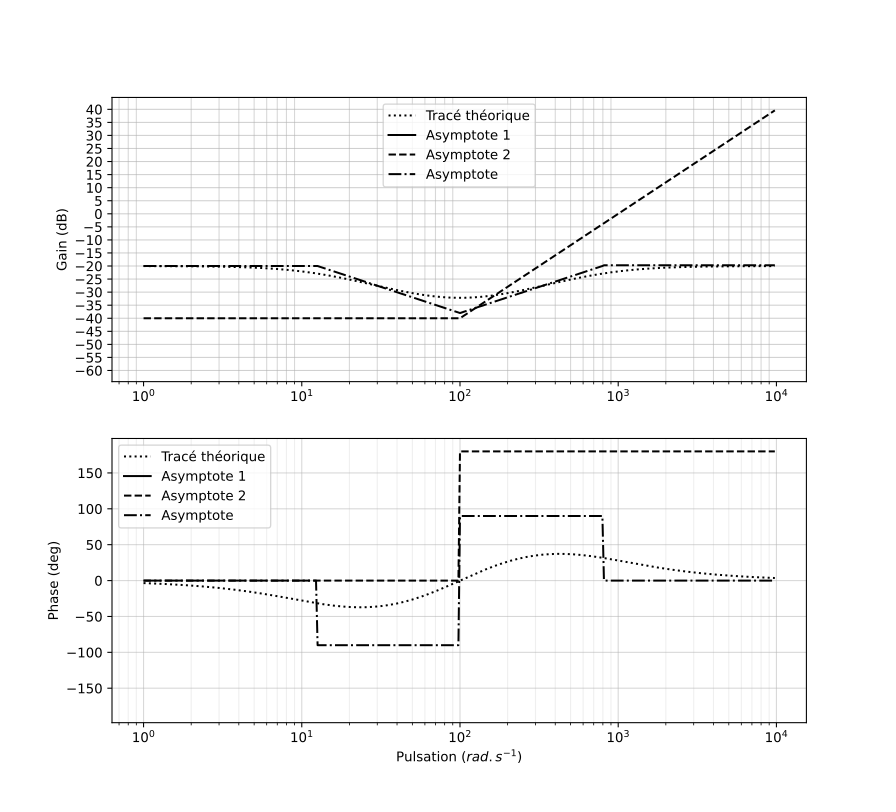
\includegraphics[width=1.1\linewidth]{img/DR_bode1}
\end{center}}{\begin{center}
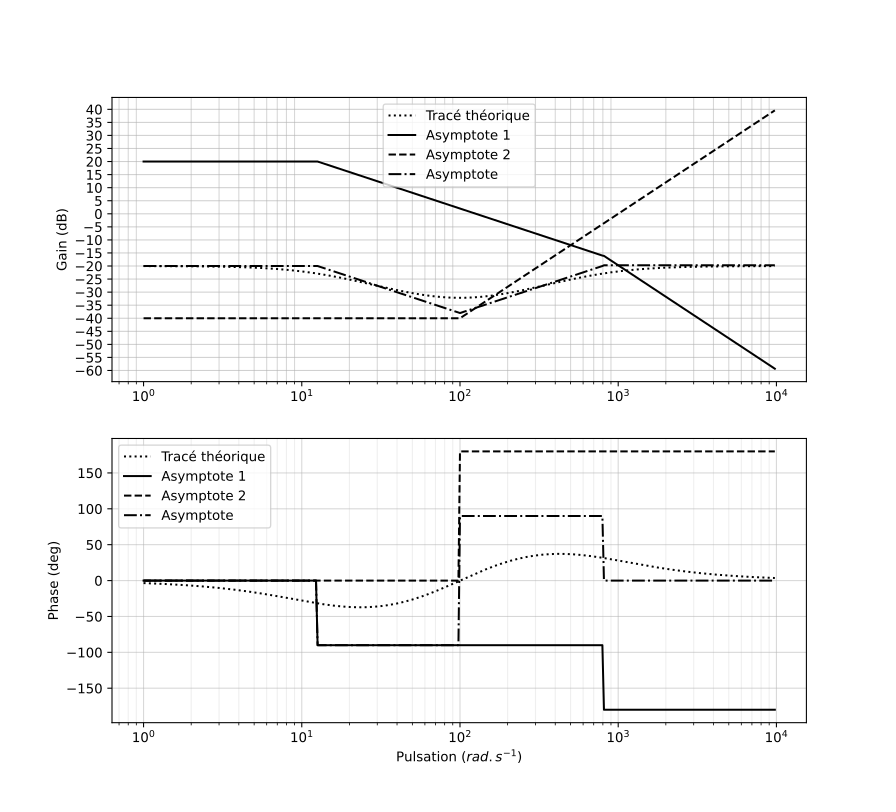
\includegraphics[width=1.1\linewidth]{img/DR_bode1_cor}
\end{center}}

\ifdef{\public}{
\vfill

\newpage}

\reponse{6}{}{
La tracé \og Asymptote 1\fg\ est celui d'un ordre 2 avec deux cassures à $\omega_1=12$ et $\omega_2=800$ et une valeur asymptotique de $20\cdot log(K)=20$, donc $K=10$,

On a donc $H_{BO1}(p)=\dfrac{10}{\left(1+\dfrac{p}{12}\right)\cdot\left(1+\dfrac{p}{800}\right)}$

Donc, la fonction de transfert est :\\$H_{BO}(p)=H_{BO1}(p)\cdot H_{BO2}(p)=\dfrac{\left(1+\dfrac{p}{100}\right)^2}{100}\cdot \dfrac{10}{\left(1+\dfrac{p}{12}\right)\cdot\left(1+\dfrac{p}{800}\right)}=\dfrac{\left(1+\dfrac{p}{100}\right)^2}{10\cdot\left(1+\dfrac{p}{12}\right)\cdot\left(1+\dfrac{p}{800}\right)}$
}

\reponse{6}{}{$\lim\limits_{\omega\rightarrow+\infty}H_{BO}(j\cdot\omega)=\dfrac{\left(\dfrac{j\cdot\omega}{100}\right)^2}{10\cdot\dfrac{j\cdot\omega}{12}\cdot\dfrac{j\cdot\omega}{800}}\approx\dfrac{1}{10}$. $20\cdot log(\dfrac{1}{10})=-20$, c'est bien ce que l'on trouve sur le tracé.}

\reponse{6}{}{Un échelon de consigne positif doit conduire à une augmentation de l'angle $\alpha$ et donc à une commande en courant $i_c(t)$ positive. $K_{jauges}$ et $K_{conv}$ étant négatif, il faut que le gain du correcteur soit aussi négatif.

$\frac{I(p)}{I_c(p)}$ de classe 0, $H_3(p)$ de classe -1 et $H_4(p) = \frac{1}{p}$. La fonction de transfert en boucle ouverte de l'asservissement en position est de classe 0. L'erreur statique est donc non nulle ; l'exigence de précision n'est pas respectée.}

\reponse{2}{\begin{center}
\def\svgwidth{\linewidth}
\input{img/DR_bode2.pdf_tex}
\end{center}}{\begin{center}
\def\svgwidth{\linewidth}
\input{img/DR_bode2_cor.pdf_tex}
\end{center}

On identifie un second ordre avec $20\cdot log(K)=60$, donc $K=1000$. $\omega_0=100rad\cdot s^{-1}$. $\xi=1$ car la valeur de la courbe est $54rad\cdot s^{-1}$ pour $\omega=\omega_0$, soit $6rad\cdot s^{-1}$ en dessous de l'asymptote. 
}

\reponse{6}{}{À $t = 0,1$ s, début de la fermeture de la pince.

À $t = 0,12$ s, la commande simule la présence de l'objet, ce qui induit un pic de courant nécessaire pour arrêter brutalement le mouvement de la pince. C'est l'effet d'un choc.

Après 0,14 s, s'établit un courant constant qui simule la réaction de l'objet sur les pinces. Cette réaction équilibre l'action de l'utilisateur.

De plus, pendant la phase de fermeture libre, entre 0,1 s et 0,12 s, on remarque une tension de commande $u_m(t)$ non nulle et positive, cohérente pour compenser la tension contre-électromotrice $e(t)$. L'intensité de consigne étant nulle, ce comportement est lié à la présence de l'intégrateur du correcteur $C_i(p)$.

Le temps de réponse à $5\%$ de l'asservissement de courant est de 0,03 s maximum. Les valeurs de tension $u_m(t)$ et d'intensité $i(t)$ ne sont effectivement pas stabilisées pendant cette phase.

Le début de la phase d'asservissement en position, à partir de $t = 0,12$ s, comprend un léger dépassement sur l'ouverture, un pic de tension et un pic d'intensité (valeur maximale admissible non atteinte).

Si le temps de réponse ne peut être caractérisé, l'ouverture prend la valeur de consigne (erreur nulle en régime permanent) malgré la perturbation $F_u$ et semble stabilisé en moins de 0,1 s.}

\sautpage{1}

~\


\end{document}
